\documentclass[10pt]{article}

\usepackage[margin=0.75in]{geometry}
\usepackage{amsmath,amsthm,amssymb}
\usepackage{xcolor}
\usepackage{cancel}
\usepackage{graphicx}
\usepackage{changepage}
\usepackage{circuitikz}
\usepackage{pgfplots}
\usepackage{physics}
\usepackage{hyperref}
\usepackage{siunitx}
\usepackage[breakable]{tcolorbox}
\usepackage[inline]{enumitem}

\theoremstyle{definition}
\newtheorem{problem}{Problem}
\newtheorem{soln}{Solution}

\pgfplotsset{compat=newest}
\usetikzlibrary{lindenmayersystems}
\usetikzlibrary{arrows}

\definecolor{incolor}{HTML}{303F9F}
\definecolor{outcolor}{HTML}{D84315}
\definecolor{cellborder}{HTML}{CFCFCF}
\definecolor{cellbackground}{HTML}{F7F7F7}
\newcommand{\eq}{=}
\usetikzlibrary{positioning, fit, calc}
\pgfdeclarelayer{background}  
\pgfsetlayers{background,main}

\makeatletter
\newcommand{\boxspacing}{\kern\kvtcb@left@rule\kern\kvtcb@boxsep}
\makeatother
\newcommand{\prompt}[4]{
    \ttfamily\llap{{\color{#2}[#3]:\hspace{3pt}#4}}\vspace{-\baselineskip}
}

\newcommand{\thevenin}[2]{
  \begin{center}
    \begin{circuitikz} \draw
      (0,0) -- (2,0) to[battery1, l_=$V_{Th}\eq#1$] (2,2) 
      to[resistor, l_=$R_{Th}\eq#2$] (0,2)
      ;
      \draw [o-] (-.07,2.079);
      \draw [o-] (-.07,0.079);
    \end{circuitikz}
  \end{center}
}

\newcommand{\norton}[2]{
  \begin{center}
    \begin{circuitikz} \draw
      (0,0) -- (3,0) to[american current source, l_=$I_{N}\eq#1$] (3,2) -- (0,2) (2,0)
      to[resistor, l=$R_{N}\eq#2$] (2,2)
      ;
      \draw [o-] (-.07,2.079);
      \draw [o-] (-.07,0.079);
    \end{circuitikz}
  \end{center}
}

\newcommand{\highlight}[1]{\colorbox{yellow}{$\displaystyle #1$}}

\hypersetup{
    colorlinks=true,
    linkcolor=blue,
    filecolor=magenta,      
    urlcolor=cyan,
    pdftitle={Overleaf Example},
    pdfpagemode=FullScreen,
    }

\NewDocumentCommand{\evalat}{sO{\big}mm}{%
  \IfBooleanTF{#1}
   {\mleft. #3 \mright|_{#4}}
   {#3#2|_{#4}}%
}

\title{Physics 2250: Problem Set VII}
\author{Jeremy Favro}
\date{\today}

\begin{document}

\maketitle

% % PROBLEM 1
\begin{problem}
Consider the circuit below containing an ac voltage source, $V_i=\cos\left(\frac{2\pi}{T}t\right)\unit{\volt}$,
and a triac device with a trigger voltage of $V_t=\pm1\unit{\volt}$ and holding currentthreshold of $I_H\approx100\unit{\micro\ampere}$.
$R_1=50\unit{\ohm}, R_2=10\unit{\kilo\ohm}, R_3=10\unit{\ohm}, R_L=10\unit{\ohm}$.
\begin{center} 
  \begin{circuitikz}
    \draw (0,0) to[american voltage source, l=$V_i$, invert] ++(0,3) to[resistor, l_=$50\unit{\ohm}$] ++(2,0)
    ++(-2,0) -- ++(0,0.5) to[resistor, l=$10\unit{\kilo\ohm}$] ++(2,0) -- ++(0,-0.5) to[resistor, l_=$10\unit{\ohm}$, n=RD] ++(0,-3) coordinate(J)
    ++(0,3) -- ++(2.5,0) to[/tikz/circuitikz/bipoles/length=1.75cm, full triac, invert, mirror, n=TR] ++(0,-3) coordinate (J1) (TR.G) -- (TR.G -| RD.left)
    (J1) to[resistor, l_=$10\unit{\ohm}$] (J) -- (0,0)
    ;

  \end{circuitikz}
\end{center}
\end{problem}
\begin{soln} 
  $$V_T=V_i-I_i\left(R_1^{-1}+R_2^{-1}\right)^{-1}$$
  $$I_L=I_i\left(\frac{R_3}{R_3+R_L}\right)$$
  $$I_{ion}=\frac{V_i}{\left(R_1^{-1}+R_2^{-1}\right)^{-1}+\left(R_L^{-1}+R_3^{-1}\right)^{-1}}=\frac{V_i}{\left(R_1^{-1}+R_2^{-1}\right)^{-1}+5\unit{\ohm}}$$
  $$I_{ioff}=\frac{V_i}{\left(R_1^{-1}+R_2^{-1}\right)^{-1}+R_3}=\frac{V_i}{\left(R_1^{-1}+R_2^{-1}\right)^{-1}+10\unit{\ohm}}$$
  $\cos(2\pi t)$ will start high, eg at $6\unit{\volt}$ which logically means the device will turn on immediately
  which means a current of $\frac{V_i}{\left(R_1^{-1}+R_2^{-1}\right)^{-1}+5\unit{\ohm}}\left(\frac{R_3}{R_3+R_L}\right)=\frac{6\unit{\volt}}{2\cdot(49.75\unit{\ohm}+5\unit{\ohm})}=\frac{4}{73}\unit\ampere$.
  This (time-variant) current will continue to flow until $\cos\left(2\pi t\right)\approx 0$ at which point the triac will shut off as both current and gate voltage have dropped below their thresholds.
  The triac will next reactivate when $6\cos\left(2\pi t\right)\left(1-\frac{\left(R_1^{-1}+R_2^{-1}\right)^{-1}}{\left(R_1^{-1}+R_2^{-1}\right)^{-1}+10\unit{\ohm}}\right)=-1\unit{\volt}$
  and will remain active until the current again reaches $\approx0\unit{\ampere}$. Then, the triac will reactivate at $V_t=1\unit{\volt}$ and the cycle repeats from there.

  \begin{center}
    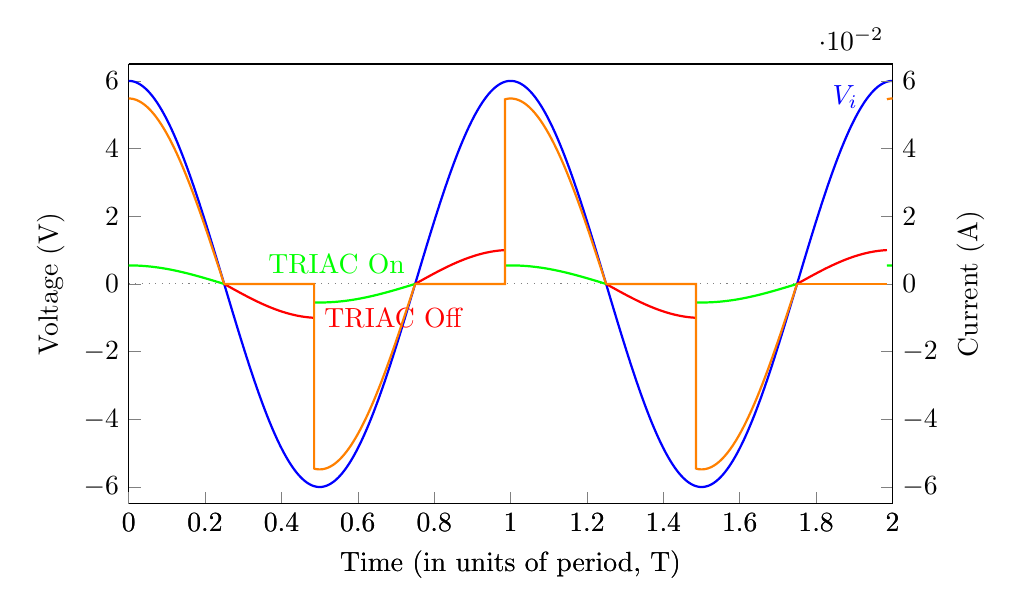
\begin{tikzpicture}[]
      \pgfplotsset{
        scale only axis,
        xmin=0, xmax=2, width=.8\linewidth,height=.2\paperheight
      }
      \begin{axis}[
          axis y line*=left,
          ymin=-6.5, ymax=6.5,
          xlabel={Time (in units of period, T)},
          ylabel={Voltage ($\unit{\volt}$)},
          xtick pos=left,
          ytick pos=left
        ]

        \addplot[thick,blue,samples=500,domain=0:2] (\x,{6*cos((2*pi*\x)*180/pi)}) node[pos=0.99, left]{$V_i$};
        \addplot[gray,dotted,samples=2,domain=0:2] (\x,{0});

        \addplot[thick,green,samples=100,domain=0:1/4] (\x,{(40/73)*cos((2*pi*\x)*180/pi)}); % on
        \addplot[thick,red,samples=100,domain=1/4:0.48547] (\x,{(240/239)*cos((2*pi*\x)*180/pi)}) node[right]{TRIAC Off}; % off
        % \addplot[thick,green,samples=500,domain=0.4:0.6] (\x,{-4/73}) node[right]{$-\frac{4}{73}\unit\ampere$};
        \addplot[thick,green,samples=100,domain=0.48547:0.75] (\x,{(40/73)*cos((2*pi*\x)*180/pi)}) node[above left]{TRIAC On};
        \addplot[thick,red,samples=100,domain=0.75:0.98547] (\x,{(240/239)*cos((2*pi*\x)*180/pi)});
        \addplot[thick,green,samples=100,domain=0.98547:1.25] (\x,{(40/73)*cos((2*pi*\x)*180/pi)});
        \addplot[thick,red,samples=100,domain=1.25:1.48547] (\x,{(240/239)*cos((2*pi*\x)*180/pi)});
        \addplot[thick,green,samples=100,domain=1.48547:1.75] (\x,{(40/73)*cos((2*pi*\x)*180/pi)});
        \addplot[thick,red,samples=100,domain=1.75:1.98547] (\x,{(240/239)*cos((2*pi*\x)*180/pi)});
        \addplot[thick,green,samples=100,domain=1.98547:2] (\x,{(40/73)*cos((2*pi*\x)*180/pi)});
        % \addplot[thick,green,samples=500,domain=0.9:1.1] (\x,{4/73}) node[right]{$\frac{4}{73}\unit\ampere$};
      \end{axis}

      \begin{axis}[
          axis y line*=right,
          ymin=-0.065, ymax=0.065,
          xlabel={Time (in units of period, T)},
          ylabel={Current ($\unit{\ampere}$)},
          xtick pos=left,
          ytick pos=right
        ]

        \addplot[thick,orange,samples=100,domain=0:1/4] (\x,{(4/73)*cos((2*pi*\x)*180/pi)}); % on
        \addplot[thick,orange,samples=100,domain=1/4:0.48547] (\x,{0}) -- (0.48547,-0.0547945205479); % off
        % \addplot[thick,green,samples=500,domain=0.4:0.6] (\x,{-4/73}) node[right]{$-\frac{4}{73}\unit\ampere$};
        \addplot[thick,orange,samples=100,domain=0.48547:0.75] (\x,{(4/73)*cos((2*pi*\x)*180/pi)});
        \addplot[thick,orange,samples=100,domain=0.75:0.98547] (\x,{0}) -- (0.98547,0.0547945205479);
        \addplot[thick,orange,samples=100,domain=0.98547:1.25] (\x,{(4/73)*cos((2*pi*\x)*180/pi)});
        \addplot[thick,orange,samples=100,domain=1.25:1.48547] (\x,{0}) -- (1.48547,-0.0547945205479);
        \addplot[thick,orange,samples=100,domain=1.48547:1.75] (\x,{(4/73)*cos((2*pi*\x)*180/pi)});
        \addplot[thick,orange,samples=100,domain=1.75:1.98547] (\x,{0});
        \addplot[thick,orange,samples=100,domain=1.98547:2] (\x,{(4/73)*cos((2*pi*\x)*180/pi)});
        % \addplot[thick,green,samples=500,domain=0.9:1.1] (\x,{4/73}) node[right]{$\frac{4}{73}\unit\ampere$};
      \end{axis}
    \end{tikzpicture}
  \end{center}
\end{soln}

% PROBLEM 2
\begin{problem}
The circuit shown below controls the brightness of a smartphone screen (via $R_L$). It
works such that when the photoconductive cell detects a high level of ambient light
(e.g., when you are out in the sun) the base-emitter junction of the transistor
becomes forward biased and automatically increases the brightness of the screen
via power expended in $R_L$. The turning on/off only depends on how the resistance
of the photoconductive cell ($R_C$) varies with the amount of light striking it.
Notes: The voltage supply is $V_{CC} = 20\unit\volt$; The resistors are: $R = 10 \unit{\kilo\ohm}$, $R_L =
  1 \unit{\kilo\ohm}$, $R_E = 2 \unit{\kilo\ohm}$; and the transistor has a forward-active working point voltage of
$V_{CE}=6\unit\volt$ and gain $\beta = 50$.
\begin{center}
  \begin{circuitikz}
    \draw \pgfextra{\ctikzset{bipoles/resistor/width=.4,
        bipoles/resistor/height=.2}} (0,0) coordinate(G) to[resistor, l=$R_E$] ++(0,1) node[npn, anchor=E](T){}
    (T.base) -- ++(-1,0) coordinate(R) to[resistor, l=$R_1$] ++(0,-1) |- (G)
    (R) to[/tikz/circuitikz/bipoles/length=30pt, ldR] ++(0,1) -- ++(0,1) coordinate(R1) -- (R1 -| T.collector) to[resistor, l=$R_L$] (T.collector)
    ;
  \end{circuitikz}
\end{center}
\end{problem}
\begin{soln} ~\\
  a) We can find the Th\'evenin equivalent of the right circuit with $R_{Th}=R_b=\frac{R_xR_1}{R_x+R_1}$ (I used $R_x$ because I kept confusing C and L when writing this on paper) and $V_{Th}=V_{b}=\frac{V_{CC}R_1}{R_1+R_x}$.
  \begin{center}
    \begin{circuitikz}
      \draw \pgfextra{\ctikzset{bipoles/resistor/width=.4,
          bipoles/resistor/height=.2}} (0,0) coordinate(G) to[resistor, l=$R_E$] ++(0,1) node[npn, anchor=E](T){}
      (T.base) to[resistor, l_=$R_{Th}$] ++(-1,0) coordinate(R) to[battery1, l=$V_{Th}$] ++(0,-1) |- (G)
      (R1 -| T.collector) to[resistor, l=$R_L$] (T.collector)
      ;
    \end{circuitikz}
  \end{center}
  
  From there we can use KVL on the bottom loop $V_{CC}\frac{R_1}{R_1+R_x}-I_b\frac{R_xR_1}{R_x+R_1}-0.7-\left(1+\beta\right)I_bR_E
    \implies I_b=\dfrac{0.7-\frac{V_{CC}R_1}{R_1+R_x}}{-\frac{R_xR_1}{R_x+R_1}-\left(1+\beta\right)R_E}$. Now, we are looking for when the transistor activates and allows current flow through $R_L$.
  This will occur when $V_b+0.7\unit{\volt}=V_e$ whent the transistor is just barely active. I think (my understanding of transistors is still very poor) that $V_e=V_{CC}-I_CR_L-V_{CE}$ so under that slightly educated assumption
  \begin{align*}
     & \frac{V_{CC}R_1}{R_1+R_x}+0.7\unit{\volt}=V_{CC}-I_CR_L-V_{CE}                                                                             \\
     & \frac{20R_1}{R_1+R_x}+0.7\unit{\volt}=20-\beta I_bR_L-6                                                                                    \\
     & \frac{20R_1}{R_1+R_x}+0.7\unit{\volt}=20-\beta \dfrac{0.7-\frac{V_{CC}R_1}{R_1+R_x}}{-\frac{R_xR_1}{R_x+R_1}-\left(1+\beta\right)R_E}R_L-6 \\
     & \frac{20R_1}{R_1+R_x}+0.7\unit{\volt}=20-\beta \dfrac{0.7-\frac{V_{CC}R_1}{R_1+R_x}}{-\frac{R_xR_1}{R_x+R_1}-\left(1+\beta\right)R_E}R_L-6 \\
     & R_x\approx11514\unit{\ohm}
  \end{align*}
  b) It's difficult to be accurate as all the indicator lines are faded but it looks like the line fits well about a third of the way between 30 and 100 lx and at exactly $3\unit{\kilo\ohm}$
  so $\frac{3\unit{\kilo\ohm}-100\unit{\kilo\ohm}}{53\unit{\lux}-1\unit{\lux}}\approx -1865\unit{\ohm\per\lux}\implies \Omega(l)=-1865\unit{\ohm\per\lux}l+101865\unit{\ohm}$
\end{soln}

% PROBLEM 3
\begin{problem}
Consider the circuit (not) below that uses a K-type thermocouple to measure and control
the temperature of a reaction in a beaker. Power expended in the $50\unit\ohm$ load resistor
RL is used to heat the reaction beaker.
  [$V_{cc}=24\unit{\volt}$, $R=10\unit{\ohm}$, $R_f=5\unit{\kilo\ohm}$, and the BJT is made is of silicon, with an operating
    point of $V_{CE}=6 \unit\volt$, $V_F=0.7\unit\volt$, and
    $\beta=50$. A K-type thermocouple look-up voltage
    table is included in the lecture notes]
\end{problem}
\begin{soln} ~\\
a) $P=\frac{V^2}{R}=\frac{(V_{cc}-V_{ce})^2}{R_L}=3.92\unit{\watt}$\\
b) Using the lookup table a $22\unit{\degreeCelsius}$ temperature coresponds to $V_{ref}=0.879\unit{\milli\volt}$. The load resistor drops $V_e=\left(1+\beta\right)I_bR_l$
and we are looking to have an output from the subtractor op amp configuration that satisfies $V_e=V_b\implies\left(1+\beta\right)I_bR_l=\frac{R_f}{R}\left(V_{TC}-V_{set}\right)$.
To find $I_b$ we go from $V_{cc}$ to ground $V_{cc}-V_{ce}-\left(1+\beta\right)I_bR_l=0\implies I_b=7.06\unit{\milli\ampere}$
\begin{align*}
  & \left(1+\beta\right)I_bR_l=\frac{R_f}{R}\left(V_{TC}-V_{set}\right)\\
  & 51\cdot7.0588\unit{\milli\ampere}\cdot50\unit{\ohm}=\frac{5\unit{\kilo\ohm}}{10\unit{\ohm}}\left(V_{TC}+36\unit{\milli\volt}\right)\\
  & V_{TC}=0
\end{align*}
c) $V_{lookup}=V_{TC}-V_{ref}=-0.879\unit{\milli\volt}$ which doesn't really make any sense at all as when I looked up a bigger table that value coresponds to an output temperature of $-22.6687\unit{\degreeCelsius}$
which to my understanding of resistance is physically impossible. I've attached my work for this question and the others in case that helps my case here but I cannot seem to figure out getting an answer that makes sense.\\
d) 
\end{soln}
\end{document}